\chapter{Silver plating}
\label{appendix:plating}

Traditional electrodes are normally Ag--AgCl coated because of the low
electrode surface noise and half-sell potential associated with
silver. Coating soft steel or other metal based electrodes with a
stable Ag--AgCl layer will enhance the electrode quality by reducing
surface noise due to electrode surface impurities. A stable Ag--AgCl
interface between the electrode base metal and the chemically active
surface of the human skin will reduce electrode noise associated with
electrode surface metal contamination forming small localized
electro-chemical currents \cite{electrode-stability}.

Small levels of contamination on the electrode contact surface can
produce large fluctuating potentials reducing the electrode's inherent
stability lowering overall signal quality as well as the SNR.

Originally it was thought to machine the electrode from a silver
bar. This idea was quickly rejected when the cost of such a decision
became apparent. It is more cost-effective to electro-plate the base
metal electrode and then coat the resulting product with a AgCl
layer. The latter is accomplished by applying a small direct current
through a saline solution in which the electrode is suspended. This
process deposits a Ag--AgCl layer on top of the silver layer. The AgCl
coating was not attempted as the process is expensive and prone to
failure. The option to coat the Ag layer with AgCl is however available
should the need for such a requirement arise.


\section{Silver plating procedure}
\begin{figure}[htbp]
		\psfrag{Silver wire}{Silver wire}
		\psfrag{Solution}{Solution}
		\psfrag{Electrode}{Electrode}
		\psfrag{A}[][]{A}
		\psfrag{-}{--}
		\psfrag{+}{+}
		\psfrag{ip}{$i_p$}
        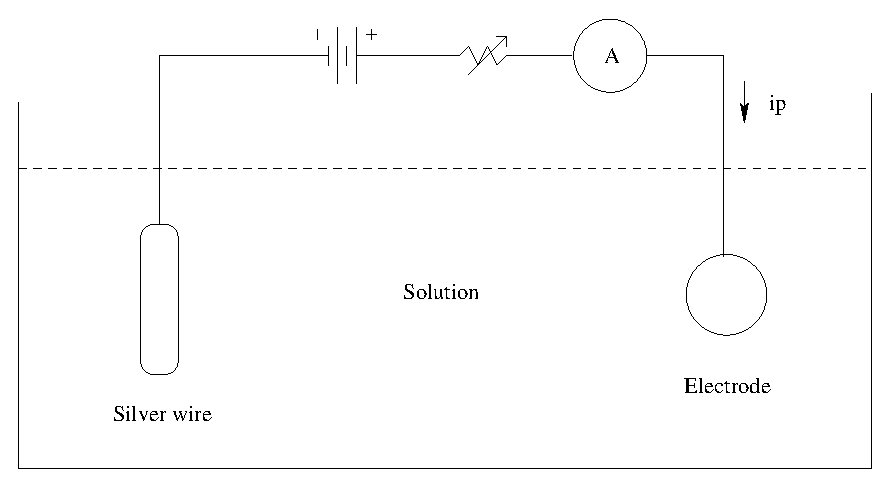
\includegraphics[width=\textwidth]{silver.eps}
        \caption{Silver coating circuit.}
        \label{fig:silver}
\end{figure}

A regulated DC power source is used to deliver approximately 5~mA to
the plating circuit, see Figure~\vref{fig:silver}. For a 5~V source a
1~k$\Omega$ resistor is used to limit the current. Either the source
potential or the series resistor value may be varied to change the
plating current. The plating current is a direct function of the
quality of the coating, a high current will result in an uneven
brittle coating cite{eeghand}. To obtain the best possible results it
is necessary to keep the plating tank at approximately 35$^0$C, keep
the current low, not exceeding 5~mA, and the tank free of foreign
metal or other contaminants.

The base metal casing is first plated with a layer of silver. This is
accomplished by suspending the casing in the plating tank solution
with preferably a platinum wire connected to the positive battery
terminal. A silver wire or rod is connected to the negative
terminal. The plating tank is filled with a silver salt solution. The
plating tank is heated to 35$^0$C while the current ($i_p$) is
carefully monitored from the ammeter. Given the area of the electrode
a period of two hours is usually sufficient time for a successful
plating procedure. Multiple electrodes may be treated at a single
session.

To coat the silver layer with AgCl the process is repeated with a AgCl
solution in the plating tank. The AgCl deposit needs to be replaced at
least once every five electro-plating procedures.


